 \documentclass[12pt,oneside]{CUNY_CS_PhD}
 \pagestyle{headings}
 \title{Reservoir Computing}
 \author{Felix Grezes}

\usepackage{fullpage}
\usepackage{graphicx}
\usepackage{amssymb}


 \begin{document}

 \frontmatter

 \maketitle 
 \makeabstractpage{Pr. Andrew Rosenberg}{  \textbf{Introduction:}
Even before Artificial Intelligence was it's own field of computational science, men have tried to mimic the activity of the human brain. In the early 1940s the first artificial neuron models were created as purely mathematical concepts. Over the years, ideas from neuroscience and computer science were used to develop the modern Neural Network. The interest in these models rose quickly but fell when they failed to be successfully applied to practical applications, and rose again in the late 2000s with the drastic increase in computing power, notably in the field of Natural Language Processing, for example with the most recent speech recognizer making heavy use of deep neural networks.\\
%This fluctuating popularity is due in large part to practical and theoretical difficulties tied to regular and Recurrent Neural Networks. With RNNs, Vanishing or ill-defined gradients, computational complexity are examples of problems that either are still unresolved or have only recently been solved. Still, since RNNs can be biologically inspired and/or approximate dynamical models, the subject has always remained interesting to the scientific community.\\
Recurrent Neural Networks (RNNs), a class of neural networks with cycles in the network, exacerbates the difficulties of traditional neural nets. Slow convergence limiting the use to small networks, and difficulty to train through gradient-descent methods because of the recurrent dynamics have limited research on RNNs, yet their biological plausibility and their capability to model dynamical systems over simple functions makes then interesting for computational researchers.\\
Reservoir Computing emerges as a solution to these problems that RNNs traditionally face. Promising to be both theoretically sound and computationally fast, Reservoir Computing has already been applied successfully to numerous fields: Natural Language Processing, Computational Biology and Neuroscience, Robotics, even Physics.\\
This survey will explore the history and appeal of both traditional feed-forward and  neural networks, before describing the theory and models of this new reservoir computing paradigm. Finally recent papers using reservoir computing in a variety of scientific field will be reviewed.
}


\tableofcontents

\mainmatter

\chapter{History of Neural Networks}
\section{Appeal and Historical Recap}
Explaining and reproducing human thought have always interested scientists and philosophers, but only with the discovery of the neuron in the 1890s by Golgi and Ram\'{o}n y Cajal, and with the advent of the computer after 1950 has it finally become a feasible goal. Today artificial intelligence is a major area of research (again to both scientists and philosophers), and artificial neural networks an important paradigm of AI.\\
An early and promising model was the perceptron, proposed in 1957 by Rosenblatt \cite{rosenblatt_perceptron_1957} of the Cornell Aeronautical Laboratory. Modeling a single neuron and using simple algorithms, the perceptron is able to learn a number of functions of its inputs. The output of the percerptron is computed as follows: $f(x) = w \cdot x + b$ where $w \cdot x$ is the dot-product of the input $x$ with the weight vector $w$ (i.e. the weighted sum of the inputs), and $b$ is a bias term.\\
However in 1969 Minsky and Papert \cite{minsky_perceptrons_1969} showed that not all functions can be learned by the perceptron, most famously the XOR () logical operation, since the perceptron is only a linear classifier. Still, research in the field stagnated until Werbos proposed the backpropagation algorithm in 1975, which solved the XOR problem by training over multiple layers of neurons. By the mid 1980s the study of artificial neural networks became a fully established field, with dedicated journals and conferences.

\section{Feed-Forward Networks: Definitions and Theory}
The fundamental building block of a neural network is the neuron. In essence the neuron is simply a model for a multivariate function whose input variables are weighted by a weight vector. Mathematically: $f(x) = \varphi(w \cdot x)$ , with $\varphi$ the chosen activation function, and $w,x$ the same as in the perceptron, i.e. respectively the weight vector and the input vector. Figure \ref{fig:neuron} gives a visualization of the artificial neuron model.\\

\begin{figure}[h]
\centering
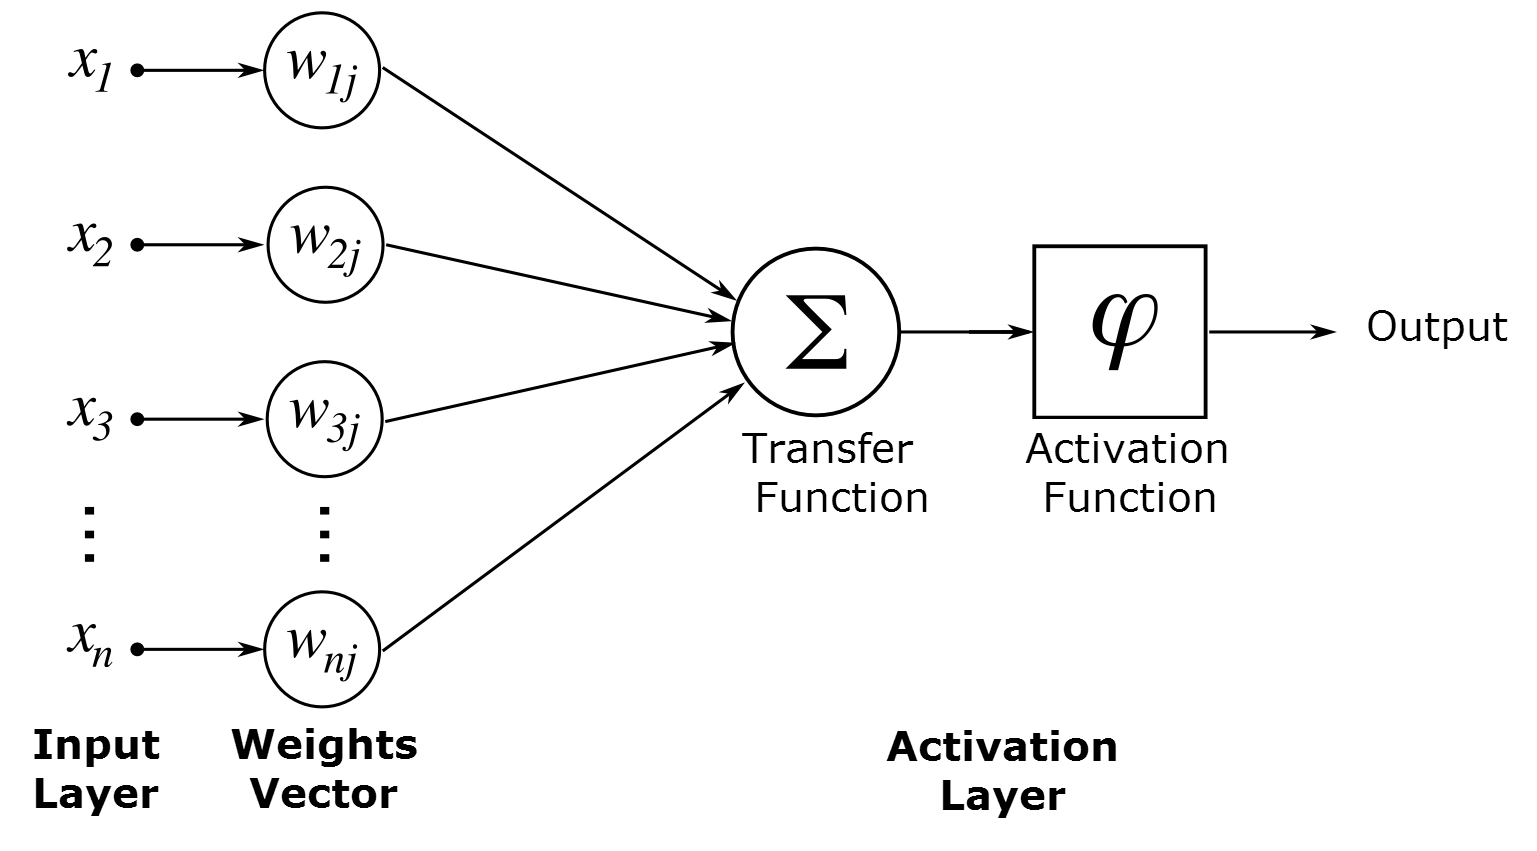
\includegraphics[width=0.9\textwidth]{pictures/ArtificialNeuronModel.png}
\caption{Model of an Artificial Neuron}
\label{fig:neuron}
\end{figure}

The transfer function is almost always summation. Some popular choices for the activation function are: threshold, linear or sigmoid; but research is also done on more esoteric activations, such as the cosine or radial functions.\\
Since the perceptron has theoretical limits, and because it is natural to do so, neurons can be combined into networks, as in the brain. The first type of network architecture we consider is the feedforward network, in which the graphical representation of the network does not contain cycles.\\
\begin{figure}[h]
\centering
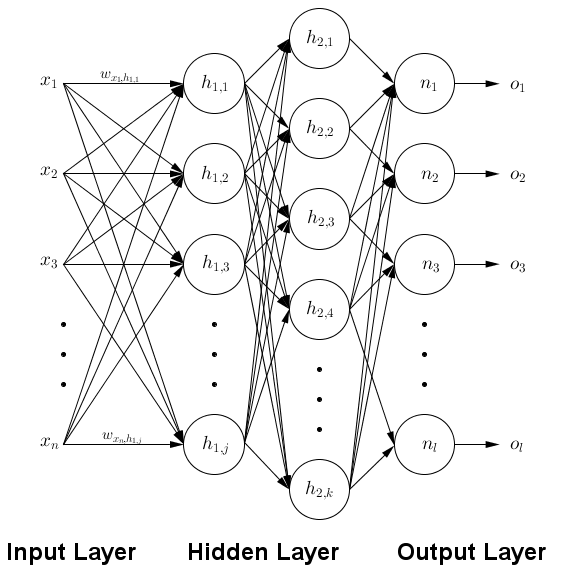
\includegraphics[width=0.9\textwidth]{pictures/FeedForwardNeuralNetwork.png}
\caption{Model of an Feedforward Neural Network}
\label{fig:feedforward}
\end{figure}
In a landmark paper, Cybenko proved in 1989 that a feedforward network containing a single hidden layer or neurons with sigmoidal activation could approximate any function of $\mathbb{R} \rightarrow \mathbb{R}$, renewing interest in the field. In 1991 Hornik proved the same for any activation function that is continuous, non-constant, bounded, and monotonically-increasing, showing that it is the multilayer feedforward architecture that provides the universal approximation power of neural networks.\\
With the theoretical hurdles surpassed, research focused on the practical application of feedforward networks. To approximate functions whose analytical form is unknown or non-existent, the proper weights have to be applied to the neuron inputs. The search for these weights is the called the training of the network, and algorithms that perform this task are often called 'learning' or 'teaching' algorithms if applied in a supervised context. The most successful of these learning algorithms is the backpropagation method, popularized by Paul Werbos in 1974.\\
The backpropagation algorithm is a variant of gradient-descent. It requires a known, desired output for each input value in order to calculate the gradient of the error and is therefore considered to be a supervised learning method. It also requires the activation function used by the neurons of the network to be differentiable.\\
The steps of the algorithm are as follows:
\begin{enumerate}
\item Forward propagation of the input values to obtain the activation of each neuron.
\item Backwards propagation of the error for each node, in order to calculate the delta for each weight.
\item Update each weight according to the gradient and to a parameter alpha (learning rate).
\item Repeat until the error over the data is below a threshold, or another criterion has been met.
\end{enumerate}
The algorithm is made possible by using the chain rule from calculus to iteratively compute gradients for each layer. Since no assumptions are made over the training dataset, it is possible to use batch, stochastic or on-line training. The main limitation of the backpropagation algorithm is the long time needed for proper training. One reason for this can be the vanishing gradient problem. If the network is too large and the learning rate inadequate, then the weights on the hidden layers closest to the input values might update too slowly for practical uses. Still, with the advances in computing power, and with multi-threaded techniques, the backpropagation algorithm has been used in recent years for speech recognition, image manipulation, medical diagnostics and more.
(see 'backpropagation' + 'field' on Google scholar for examples)

\section{Recurrent Neural Networks}
For better or for worse, part of the appeal of neural networks is the parallel with the human brain. However, the network architecture of neurons within the brain is decidedly not a feedforward architecture. Networks in which the graphical representation contains cycles are called Recurrent Neural Networks (RNNs).\\
The study of RNNs is essential to any type of research done on modelling, simulating a human or animal brain. But RNNs are not only useful due to their biological modelling capacities, but also because they have superior theoretical computational power. A feedforward network approximates a mathematical function, whereas RNNs approximate dynamical systems. Dynamical systems are essentially functions with an added time component, the same input input can result in a different output at different timesteps. It is the presence of cycles in the network that allow these dynamical changes to occur. In theory, RNNs are capable of remembering input values for some time by preserving them in some form within the activations of nodes in the network. Hopefully RNNs are capable of learning context sensitive information without having to engineer task-specific data representations as input to the network (e.g. triphones or n-grams in NLP tasks), though these can still be used with RNNs. The following picture gives a graphical example of a small RNN.\\
(pic)\\
Of course, the increased complexity of the network architecture comes at a cost. New techniques for training have to be devised, and in practical cases are almost always slower than feedforward network training algorithms. Theoretical mathematical results from feedforward networks also do not necessarily hold true for RNNs and must be proven again, if possible. The study of RNNs requires its own, tailored approach.\\
One important theoretical result came in 1991, when Siegelmann and Sontag proved that RNNs, of finite size and with sigmoidal activation function for the nodes, have the capacity to simulate a universal Turing machine, confirming the computational power of RNNs.

\subsubsection{Backpropagation through Time}
For practical applications, a successful training technique for RNNs has been Backpropagation Through Time (BPTT), which was independently derived by numerous researchers but popularized in 1991 by Paul Werbos. It is an adaptation of the well-known backpropagation training method known from feedforward networks. The feedforward backpropagation algorithm cannot be directly transferred to RNNs because the error backpropagation pass presupposes that the connections between units induce a cycle-free ordering. The solution of the BPTT approach is to "unfold" the recurrent network in time, by stacking identical copies of the RNN, and redirecting connections within the network to obtain connections between subsequent copies. This gives a feedforward network, which is compatible with the backpropagation algorithm.\\
(pic)\\
The remarks concerning the slow convergence of standard backpropagation carry over to BPTT, even more so since the size the network grows every iterations. This has limited the used of BPTT to small networks, in the order of tens or hundreds of nodes.

\chapter{The Reservoir Computing Paradigm}
In this context of difficult progress for RNNs, in 2001 a fundamentally new approach to RNN design and training was proposed independently by Wolfgang Maass under the name of Liquid State Machines and by Herbert Jaeger under the name of Echo State Networks. This approach, which had predecessors in computational neuroscience (Peter Dominey 1995) and subsequent ramifications in machine learning as the Backpropagation-Decorrelation learning rule proposed by Schiller and Steil in 2005, is now increasingly often collectively referred to as Reservoir Computing (RC).\\
As Schiller and Steil noticed, when applying BPTT training to RNNs the dominant changes appear in the weights of the output layer, while the weights of the deeper layer converged slowly. It is this observation that  motivates the fundamental idea of Reservoir Computing: if only the changes in the output layer weights are significant, then {\itshape the treatment of the weights of the inner network can be completely separated from the output layer weights.}

\section{Reservoir Models}
Reservoir computing methods differ from traditional RNN learning techniques by making a conceptual  and computational separation between the reservoir, the inner neurons and weights of the network, and the readout, the neurons and weights that produce the output. More specifically, in traditional supervised learning the error between the desired output and computed output will potentially influence the weights of all the network. By contrast, in the Reservoir Computing paradigm, the error will only influence the weights of the readout layer. The weights of the RNN itself are set at the start of the learning and do not change.
(DRAW PIC of influence of error)
Despite being a relatively new concept, the Reservoir computing paradigm has already been successfully applied to a range of scientific fields. The following are different brands of reservoir methods. Most of these techniques were developed independently and have only been united under the term Reservoir since 2008. Each brand has its own history and mindset.

\subsubsection{Echo State Networks}
The Echo State Networks (ESNs) method, created by Herbert Jaeger and his team, represents one of the two pioneering reservoir computing methods. Having observed that if a RNN possesses certain algebraic properties, then it is possible to achieve high classification performance on practical applications simply by learning a linear classifier on the readout nodes, for example using linear regression. The untrained nodes of the RNN are part of what is called the dynamical reservoir, which is where the name Reservoir Computing comes from. The Echo State names comes from the input values echoing throughout the states of the reservoir due to its recurrent nature. ESNs usually use sigmoïd neurons, but more biologically inspired models such as leaky integrator neurons have also been used.

\subsubsection{Liquid State Machines}
Liquid State Machines (LSMs) are the other pioneer method of reservoir computing, developed simultaneously and independently from Echo State Networks, by Wolfgang Maass. Coming from a computational neuroscience background, LSMs use more biologically realistic models of spiking integrate-and-fire neurons and dynamic synaptic connection models, in order to understand the computing power of real neural circuits. As such LSMs also use bio-inspired topologies and metric constraints for neuron connections in the reservoir, instead of the randomized network of ESNs. This usually makes LSMs more complicated to implement, and less useful for practical purposes.

\subsubsection{Temporal Recurrent Networks}
We should also mention Peter Dominey's decade long research on cortico-striatal circuits in the human brain. His research aims at elucidating complex neural structures rather than theoretical computational principles, but he was probably the first to properly state the Reservoir Computing principles by observing that there is no learning (adaptation) deep within the neural network, and that these connections are randomized (in the pre-frontal cortex in his case). Only in 2008 have computational researchers become aware of Dominey's work.

\subsubsection{Other Exotic Networks}
As mentioned previously, the idea of treating the reservoir and the readout layer separately was also devised by the Schiller and Steil. They proposed an algorithm called Backpropagation-Decorrelation as a new RNN training method, boasting fast convergence and good practical results. \\
The Reservoir Computing paradigm can be extended beyond neural networks. Taking the idea of a reservoir and echoes quite literally, an experiment was set up where the inputs were projected into a bucket of water, and by recording the waves bouncing around the liquid's surface, the authors were able to successfully train a pattern recognizer. Another exotici dea for an untrained reservoir is an E.Coli. bacteria colony, with chemical stimuli as input and protein measures as output.

\section{Reservoir Computing Theory}
While Reservoir Computing techniques can rely on randomized networks to obtain good performance, there is no guarantee that it is optimal. In fact 'random' is almost by definition the opposite of 'optimal'. While no single technique will work for all tasks, some general rules exist to create reservoirs with good behavior.

\subsubsection{Echo State Property}
An important element for Reservoir Computing to work , coming from the ESNs approach, is that the reservoir should have the echo state property. This condition in essence states that the effect of a previous state and a previous input on a future state should vanish gradually as time passes, and not persist or worse, get amplified. For practical purposes, the echo state property is assured if the matrix W of reservoir weights is scaled so that its spectral radius ρ(W) (i.e., the largest absolute eigenvalue) is close to or inferior to 1. Intuitively, the spectral radius is a crude measure of the amount of memory the reservoir can hold, the small values meaning a short memory, and the large values a longer memory, up to the point of over-amplification when the echo state property no longer holds.

\subsubsection{Separability Property}
Another important aspect of good reservoirs is the capacity to separate two different inputs, i.e. the output activity should differ. However this contrasts with the previously stated Echo State Property; if the two signals only vary in the very beginning, than the reservoir will eventually stabilize to the same state. Thus the separability property applies to a fixed number of timesteps. Balancing the two properties is a task-specific problem. To increase the separability of a reservoir, a good heuristic to to make the network connections sparse and random. This will  make the activation signals within the network decoupled and varied.

\subsubsection{Topology}
A larger number of neurons in the network will mean more activation signals, allowing for finer grain classification for example. Concerning the particular topology of the network, it has been noted that there is substantial variation in ESN performance among randomly created reservoirs. However, in a study of different topologies were tested, such as scale-free,small world or biologically inspired; but none tested to "perform significantly better than simple random networks". Still the difference in performance amongst these random networks indicates that similar approaches might be useful.

\subsubsection{Unsupervised reservoir adaptation}
One simple test to measure the memory capacity of a reservoir is to implement the task of recreating the input as output, with a time given time delay. This tests that the reservoirs has a  the desired memory capacity. Other tests including choosing reservoirs with minimal pair-wise activation of neurons, 


\chapter{Recent Literature Review}
This survey will first present recent scientific papers that have used the reservoir computing paradigm in the fields of applied physics, machine learning theory, computational neuroscience and robotics. It will then transition to papers more closely related to my own field, natural language processing.

\section{General Scientific Papers}
\subsection{A reservoir of time constants for memory traces in cortical neurons \cite{bernacchia_reservoir_2011}}

\subsection{Multiobjective Reinforcement Learning Using Adaptive Dynamic Programming And Reservoir Computing \cite{oubbati_multiobjective_2012}}

\subsection{Constructing optimized binary masks for reservoir computing with delay systems \cite{appeltant_constructing_2014}}

\subsection{Exploring the acquisition and production of grammatical constructions through human-robot interaction with echo state networks \cite{hinaut_exploring_2014}}

\section{Natural Language Processing Papers}
\subsection{Isolated Word Recognition with the Liquid State Machine: A Case Study \cite{verstraeten_isolated_2005}}

\subsection{Phoneme recognition with large hierarchical reservoirs \cite{triefenbach_phoneme_2010}}

\subsection{Connected digit recognition by means of reservoir computing \cite{jalalvand_connected_2011}}

\subsection{On-Line Processing of Grammatical Structure Using Reservoir Computing \cite{hinaut_-line_2012}}


\chapter{Other Randomized Networks}

\chapter{Conclusion and my own future work}

\backmatter

\bibliographystyle{ieeetr}
\bibliography{bibl}
\addcontentsline{toc}{chapter}{\numberline{}Bibliography }

\end{document}